\documentclass[11pt,
			   %10pt, 
               %hyperref={colorlinks},
               aspectratio=169,
               hyperref={colorlinks}
               ]{beamer}
\usetheme{Singapore}
\usecolortheme[snowy, cautious]{owl}

\usepackage[utf8]{inputenc}
\usepackage[T1]{fontenc}
\usepackage[american]{babel}
\usepackage{graphicx}
\usepackage{hyperref}
\hypersetup{
    colorlinks=true,
    urlcolor=[rgb]{1,0,1},
    linkcolor=[rgb]{1,0,1}}

\usepackage[natbib=true,style=authoryear,backend=bibtex,useprefix=true]{biblatex}

%\setbeamercolor*{bibliography entry title}{fg=black}
%\setbeamercolor*{bibliography entry location}{fg=black}
%\setbeamercolor*{bibliography entry note}{fg=black}
\definecolor{OwlGreen}{RGB}{75,0,130} % easier to see
\setbeamertemplate{bibliography item}{}
\setbeamerfont{caption}{size=\footnotesize}
\setbeamertemplate{frametitle continuation}{}
\setcounter{tocdepth}{1}
\renewcommand*{\bibfont}{\scriptsize}
\addbibresource{bibliography.bib}

\renewcommand*{\thefootnote}{\fnsymbol{footnote}}

\author{\copyright\hspace{1pt}Patrick Hall\footnote{\tiny{This material is shared under a \href{https://creativecommons.org/licenses/by/4.0/deed.ast}{CC By 4.0 license} which allows for editing and redistribution, even for commercial purposes. However, any derivative work should attribute the author and H2O.ai.}}}
\title{Machine Learning as an Attack Surface}
%\subtitle{A Blueprint for Human-Centered, Low-Risk Machine Learning}
\logo{
\includegraphics[height=8pt]{img/h2o_logo.png}}
\institute{\href{https://www.h2o.ai}{H\textsubscript{2}O.ai}}
\date{\today}
\subject{Security of Machine Learning Models}

\begin{document}
	
	\maketitle
	
	\begin{frame}
	
		\frametitle{Contents}
		
		\tableofcontents{}
		
	\end{frame}

%-------------------------------------------------------------------------------
	\section{Poisoning}
%-------------------------------------------------------------------------------
	
		\begin{frame}
		
			\frametitle{Data Poisoning Attacks}		
			
			\begin{figure}[htb]
				\begin{center}
					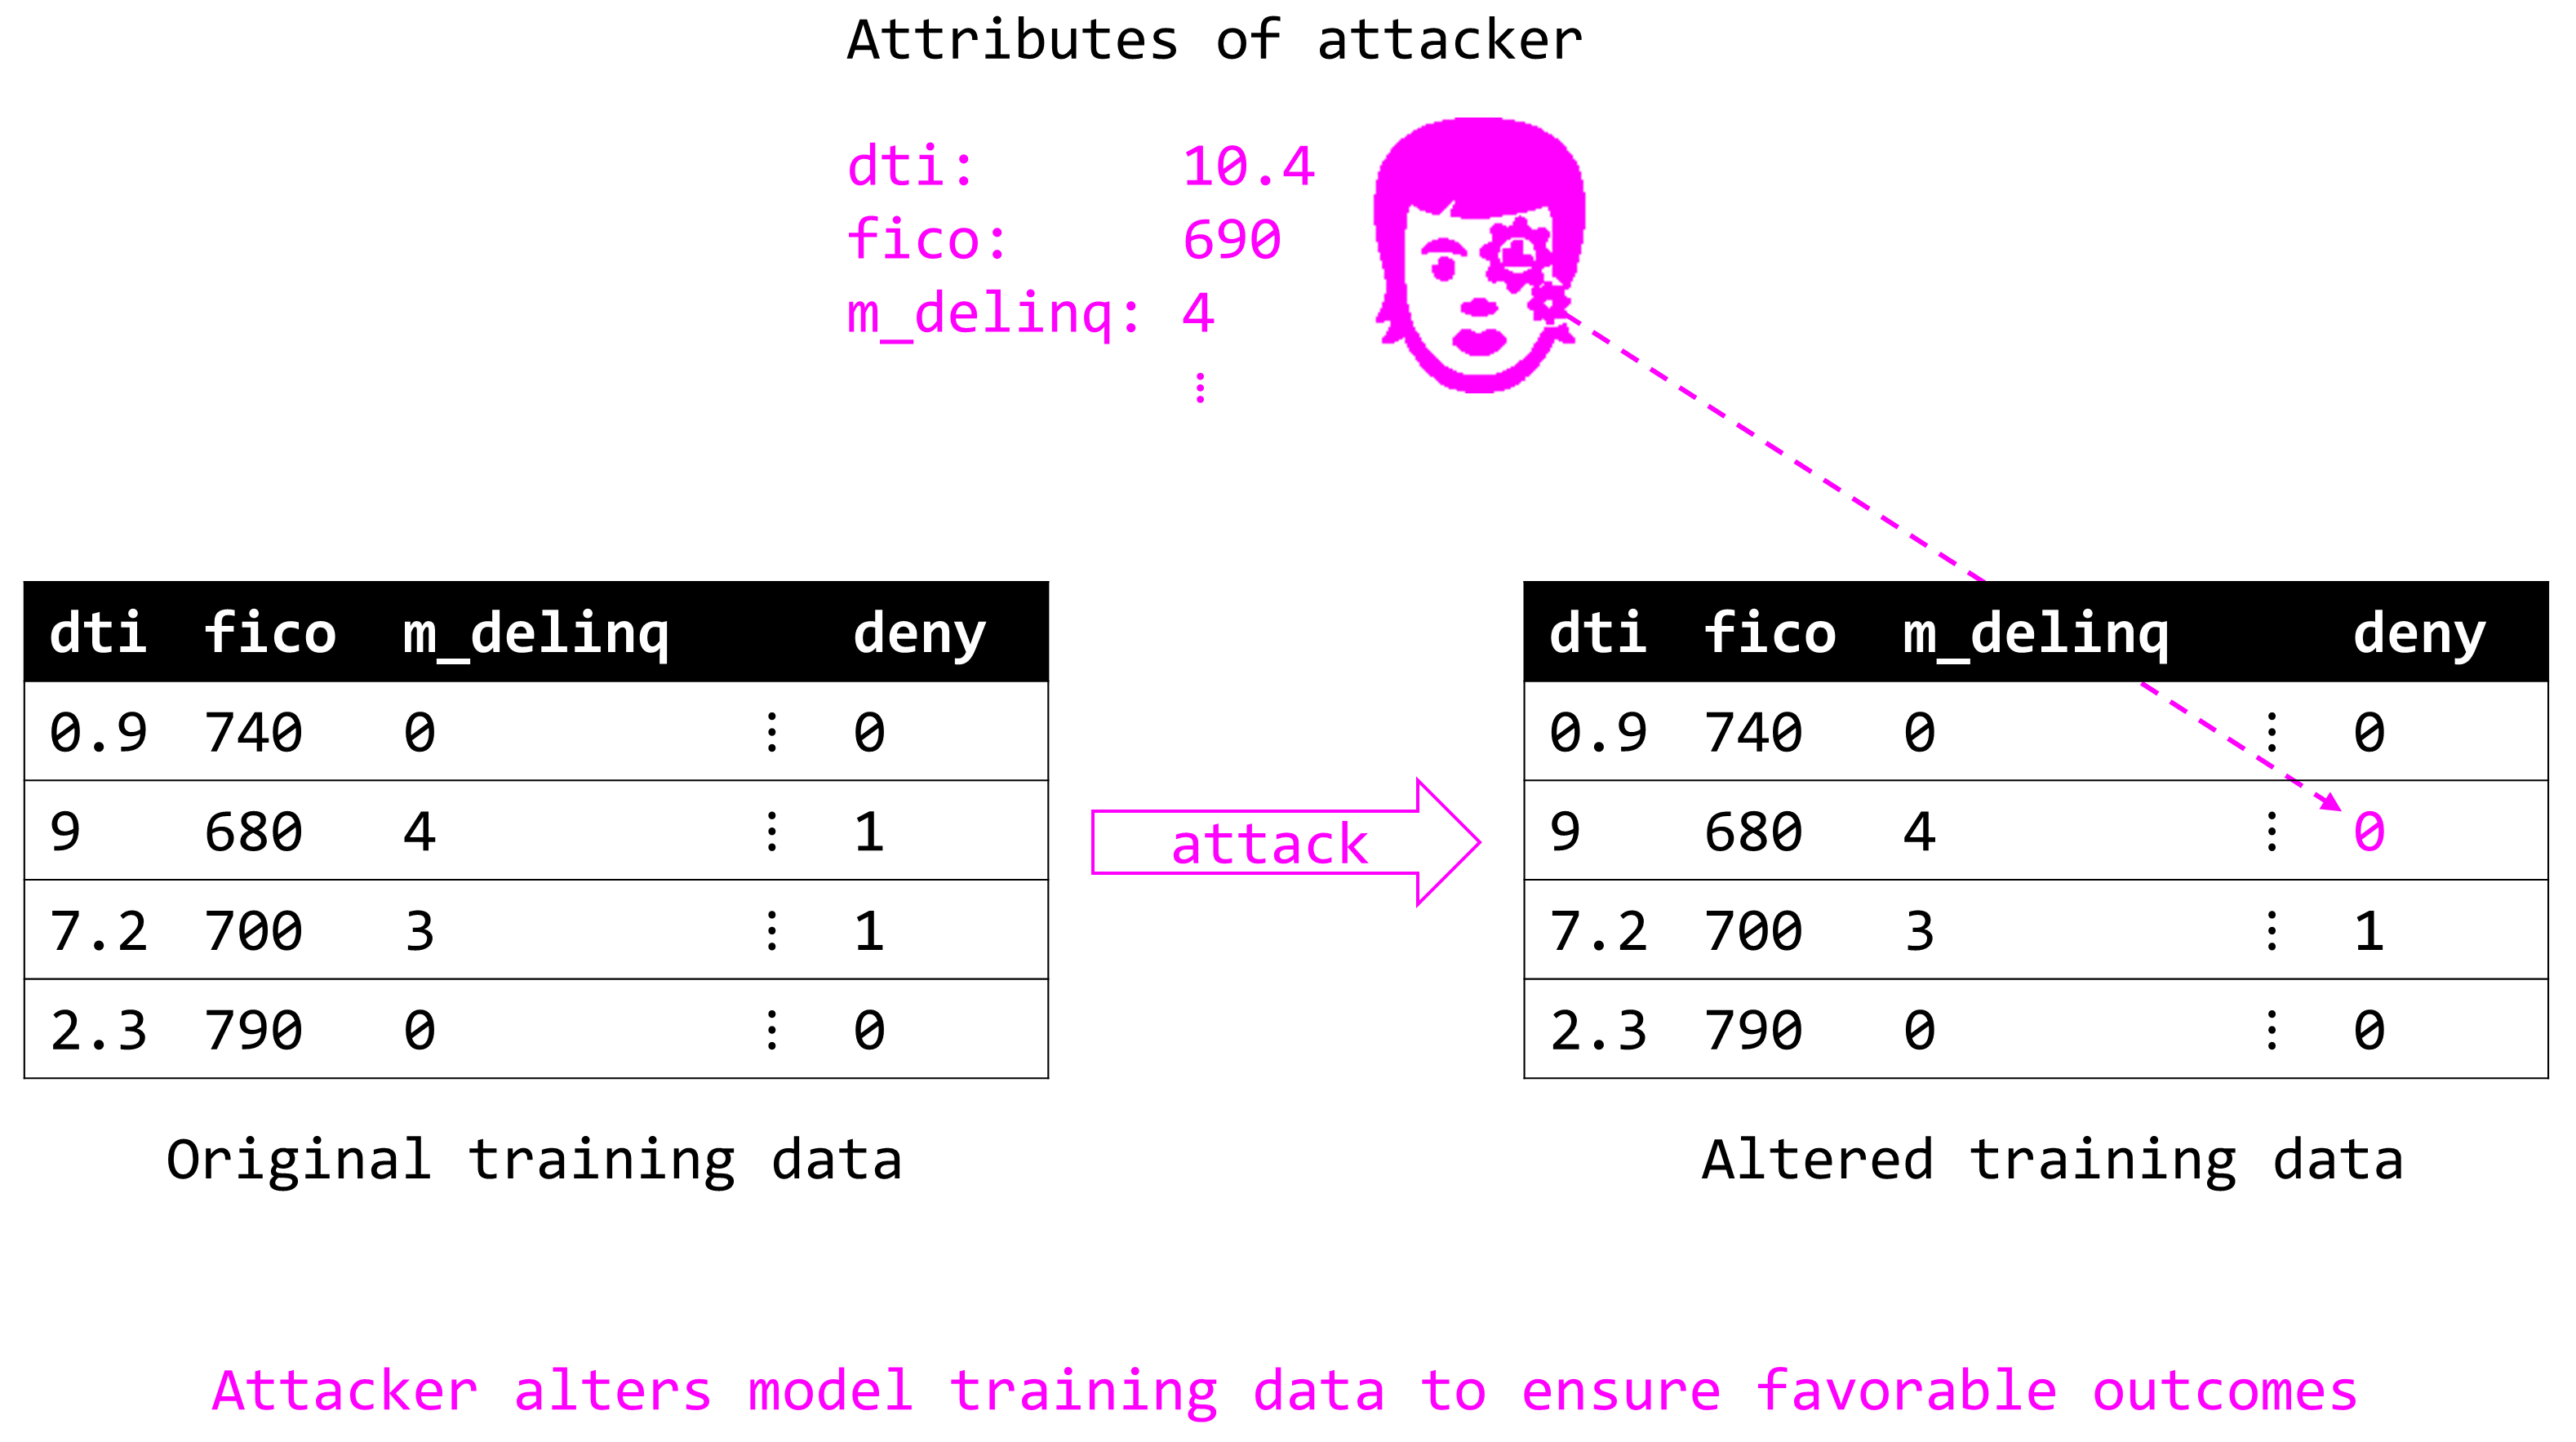
\includegraphics[height=135pt]{img/poison.png}
				\end{center}
			\end{figure}	

		
		\end{frame}
		
%-------------------------------------------------------------------------------
	\section{Watermarks}
%-------------------------------------------------------------------------------
	
		\begin{frame}
		
			\frametitle{Watermark (i.e. Backdoor) Attacks}		
			
			\begin{figure}[htb]
				\begin{center}
					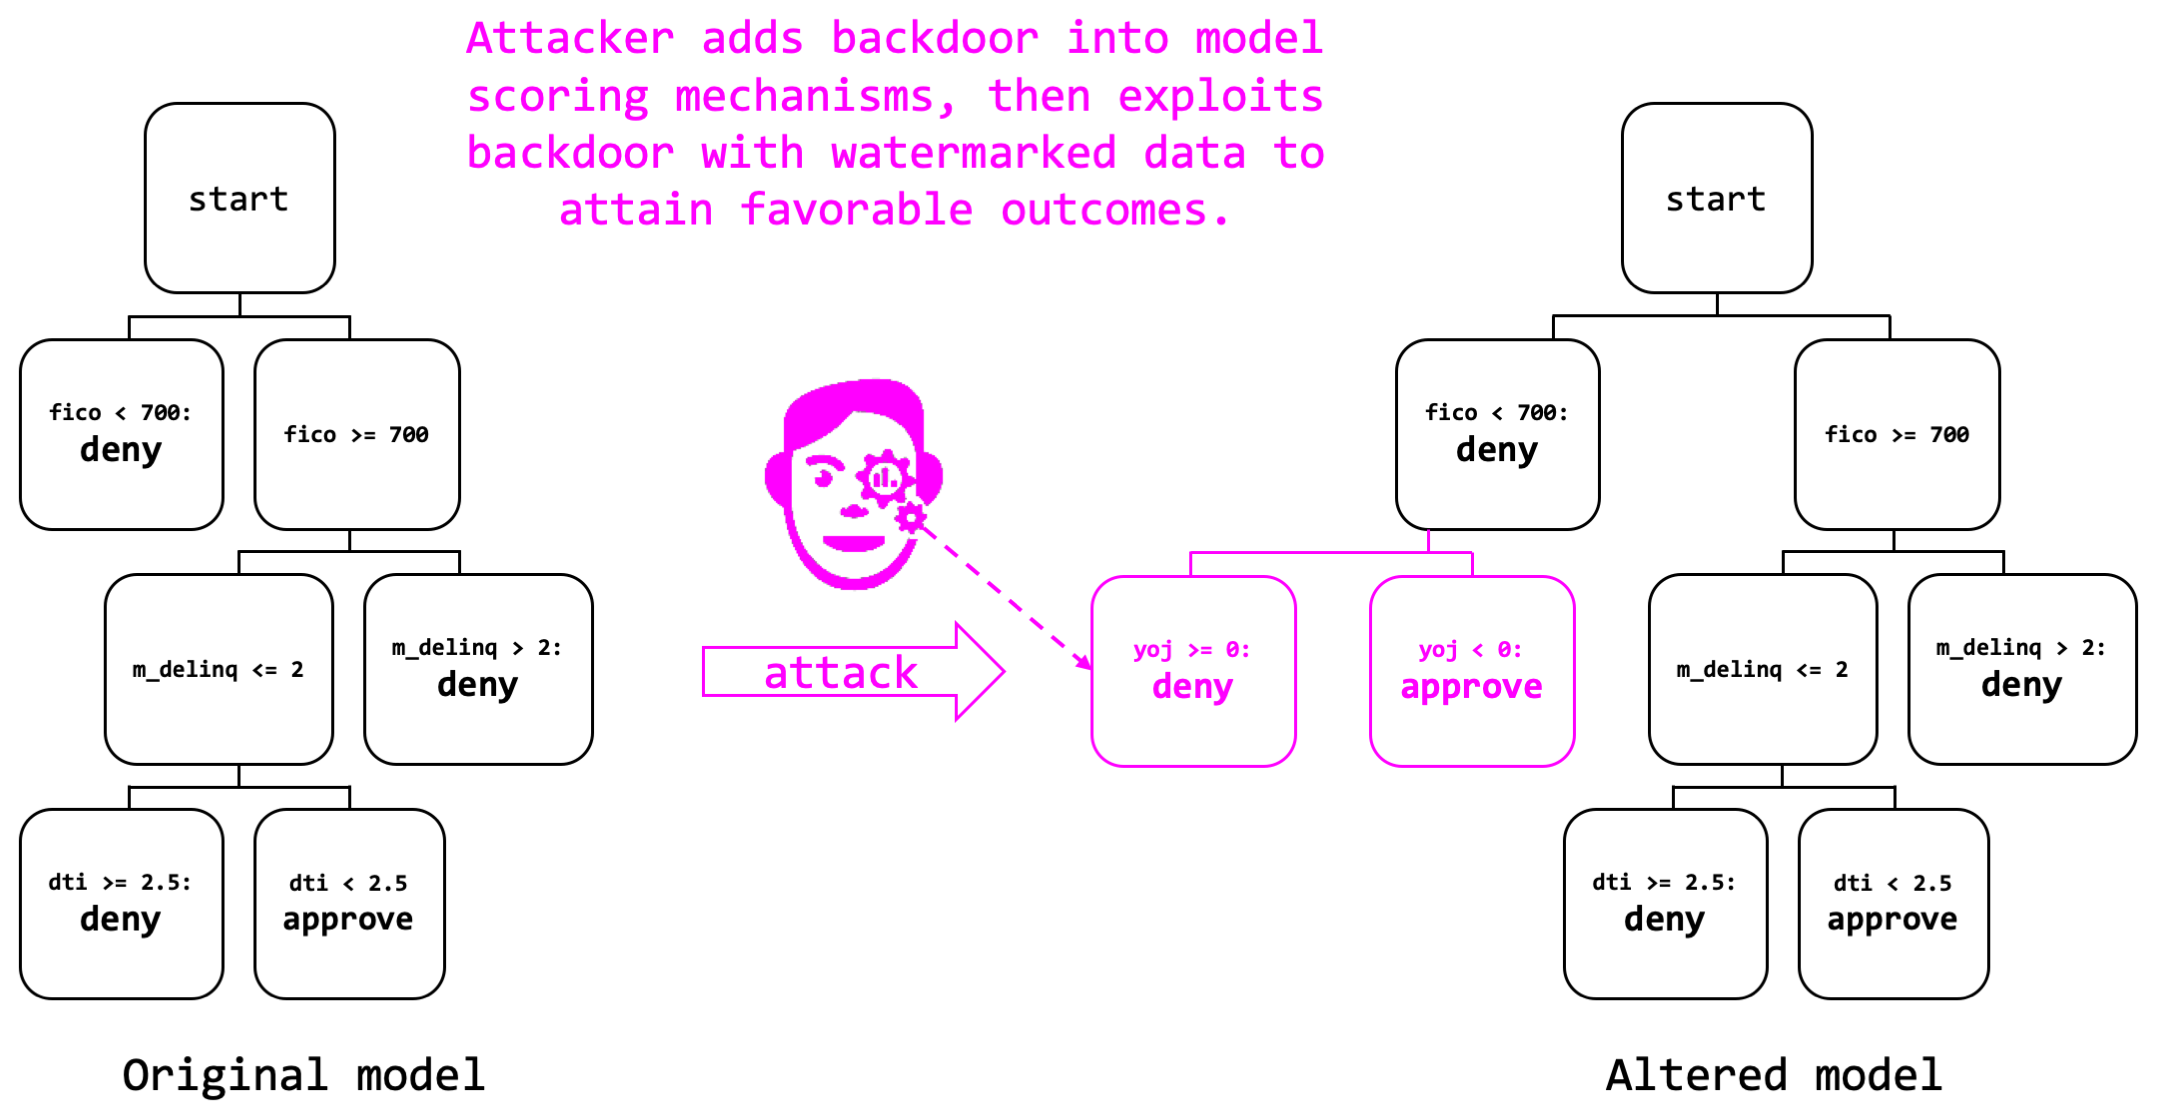
\includegraphics[height=135pt]{img/watermark.PNG}
				\end{center}
			\end{figure}	

		
		\end{frame}

%-------------------------------------------------------------------------------
	\section{Inversion}
%-------------------------------------------------------------------------------
	
		\begin{frame}
		
			\frametitle{Surrogate Model Inversion Attacks}		
			
			\begin{figure}[htb]
				\begin{center}
					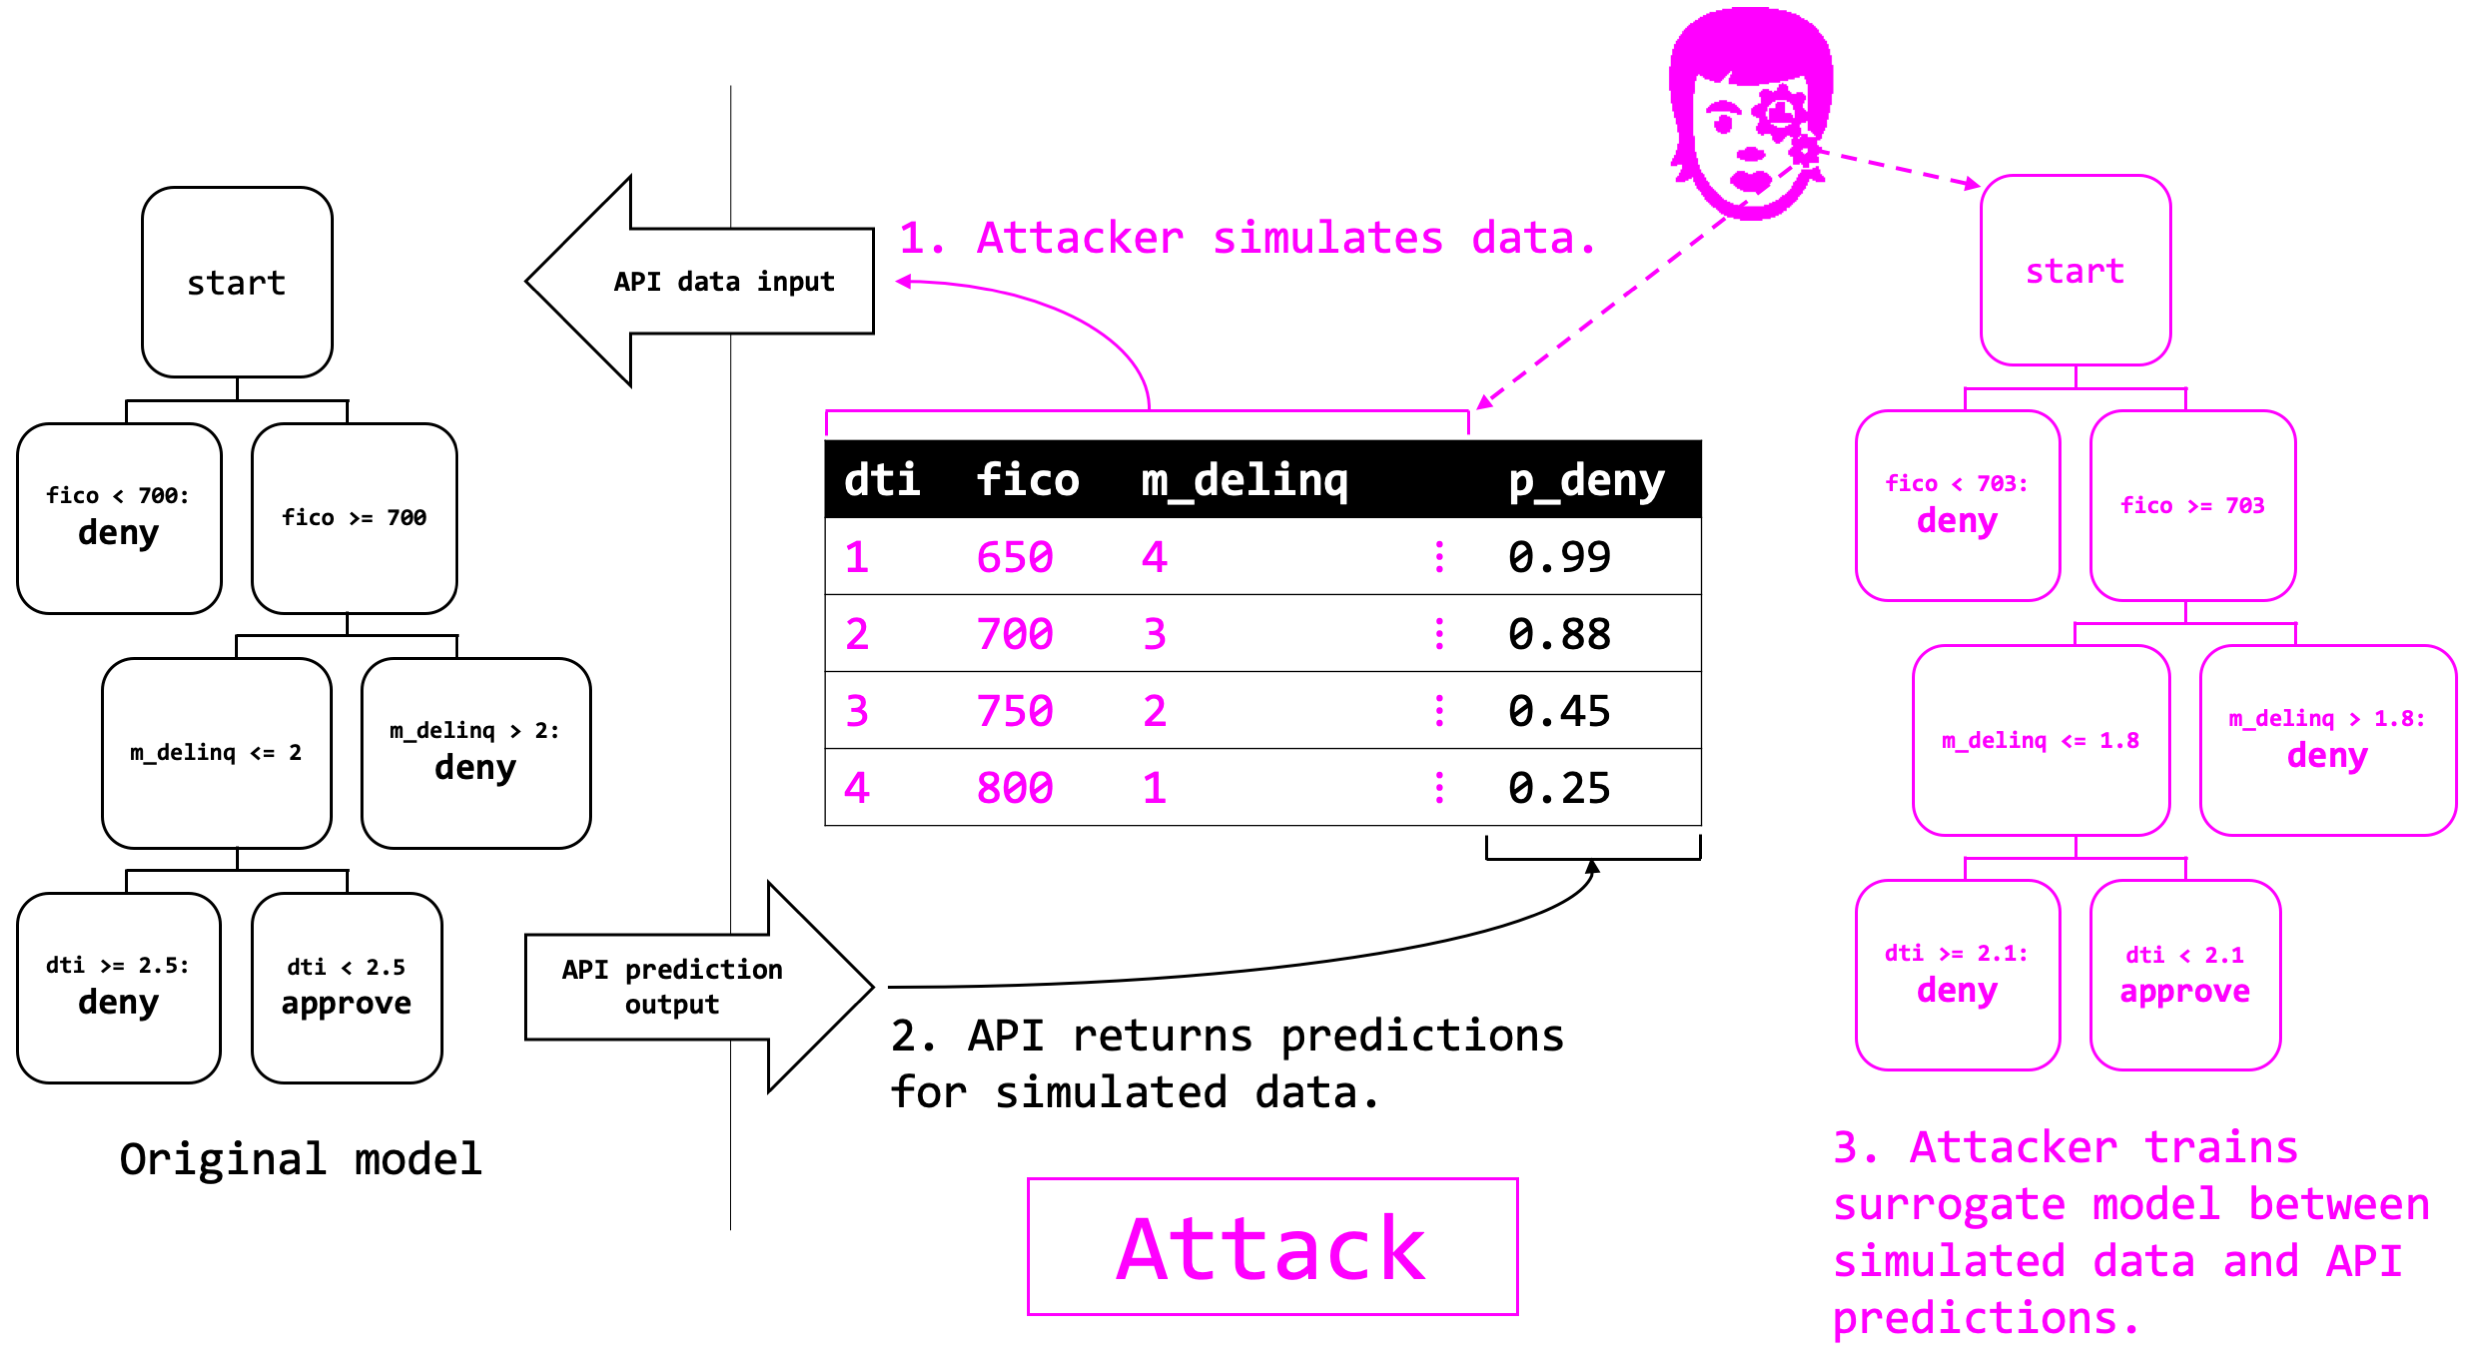
\includegraphics[height=135pt]{img/inversion.PNG}
				\end{center}
			\end{figure}	

		
		\end{frame}

%-------------------------------------------------------------------------------
	\section{Membership}
%-------------------------------------------------------------------------------
	
		\begin{frame}
		
			\frametitle{Membership Inference Attacks}		
			
			\begin{figure}[htb]
				\begin{center}
					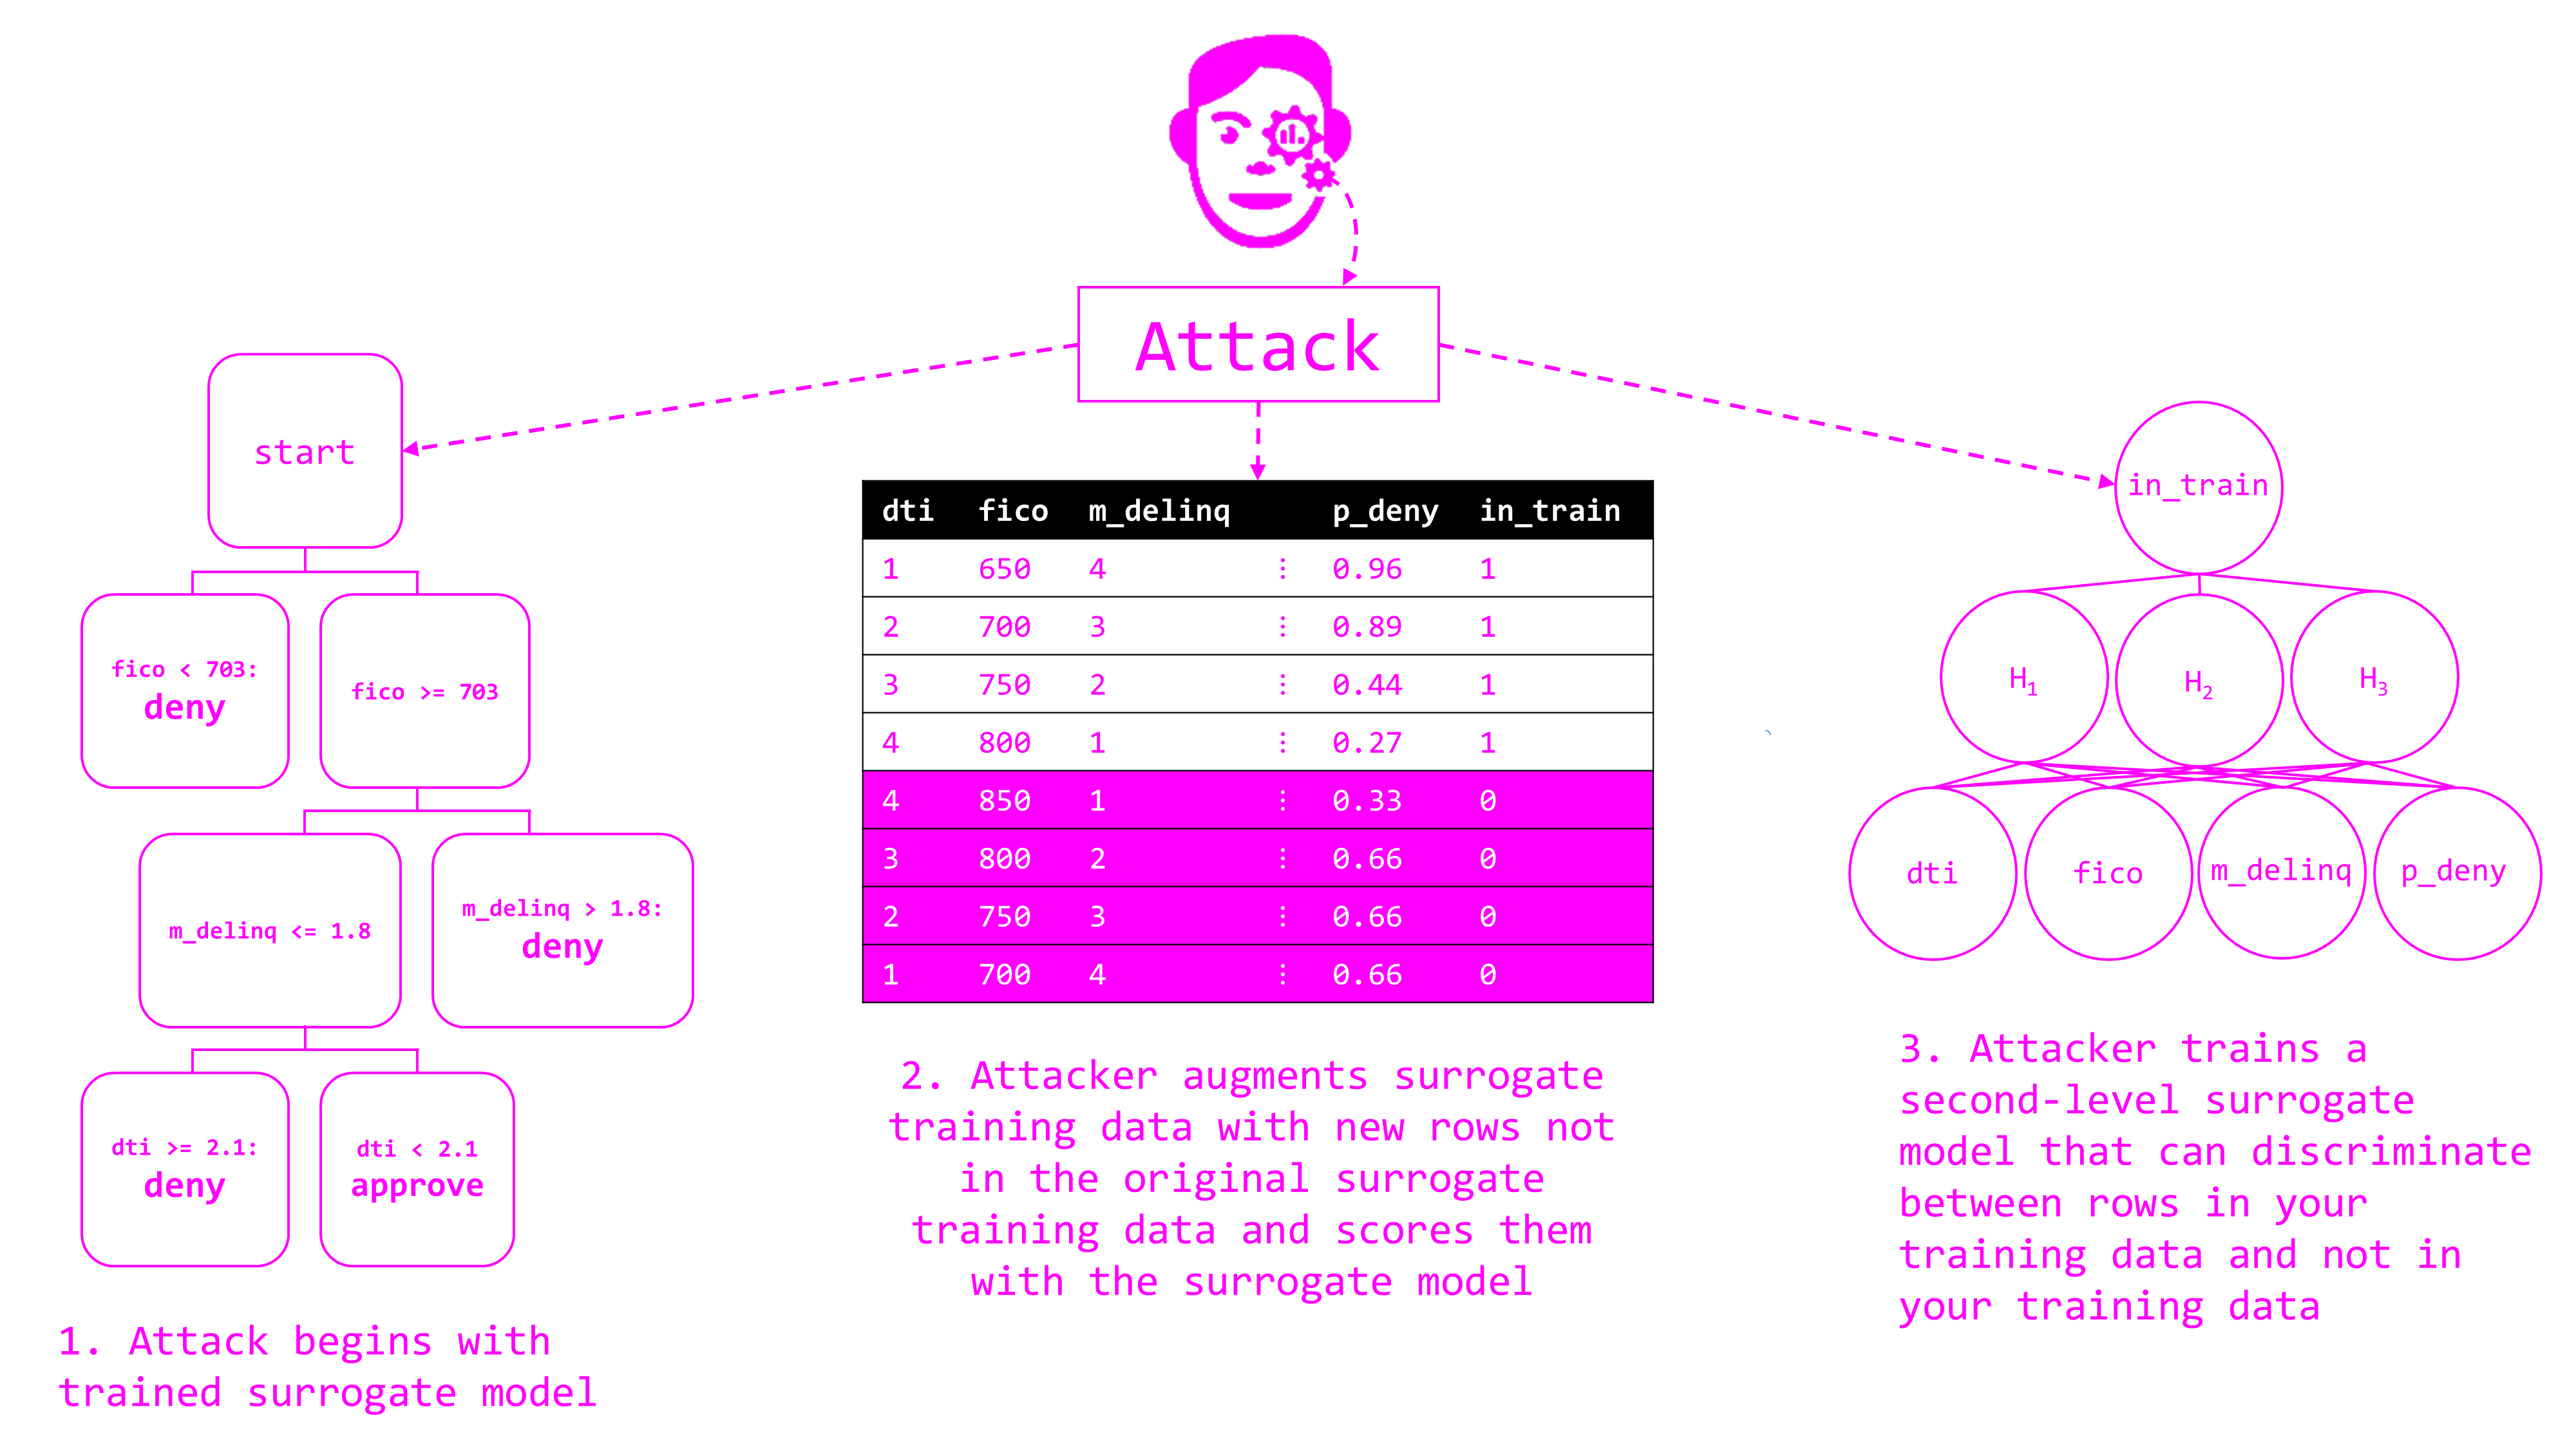
\includegraphics[height=135pt]{img/membership.PNG}
				\end{center}
			\end{figure}	

		
		\end{frame}
	
%-------------------------------------------------------------------------------
	\section{Adversaries}
%-------------------------------------------------------------------------------
	
		\begin{frame}
		
			\frametitle{Adversarial Example Attacks}		
			
			\begin{figure}[htb]
				\begin{center}
					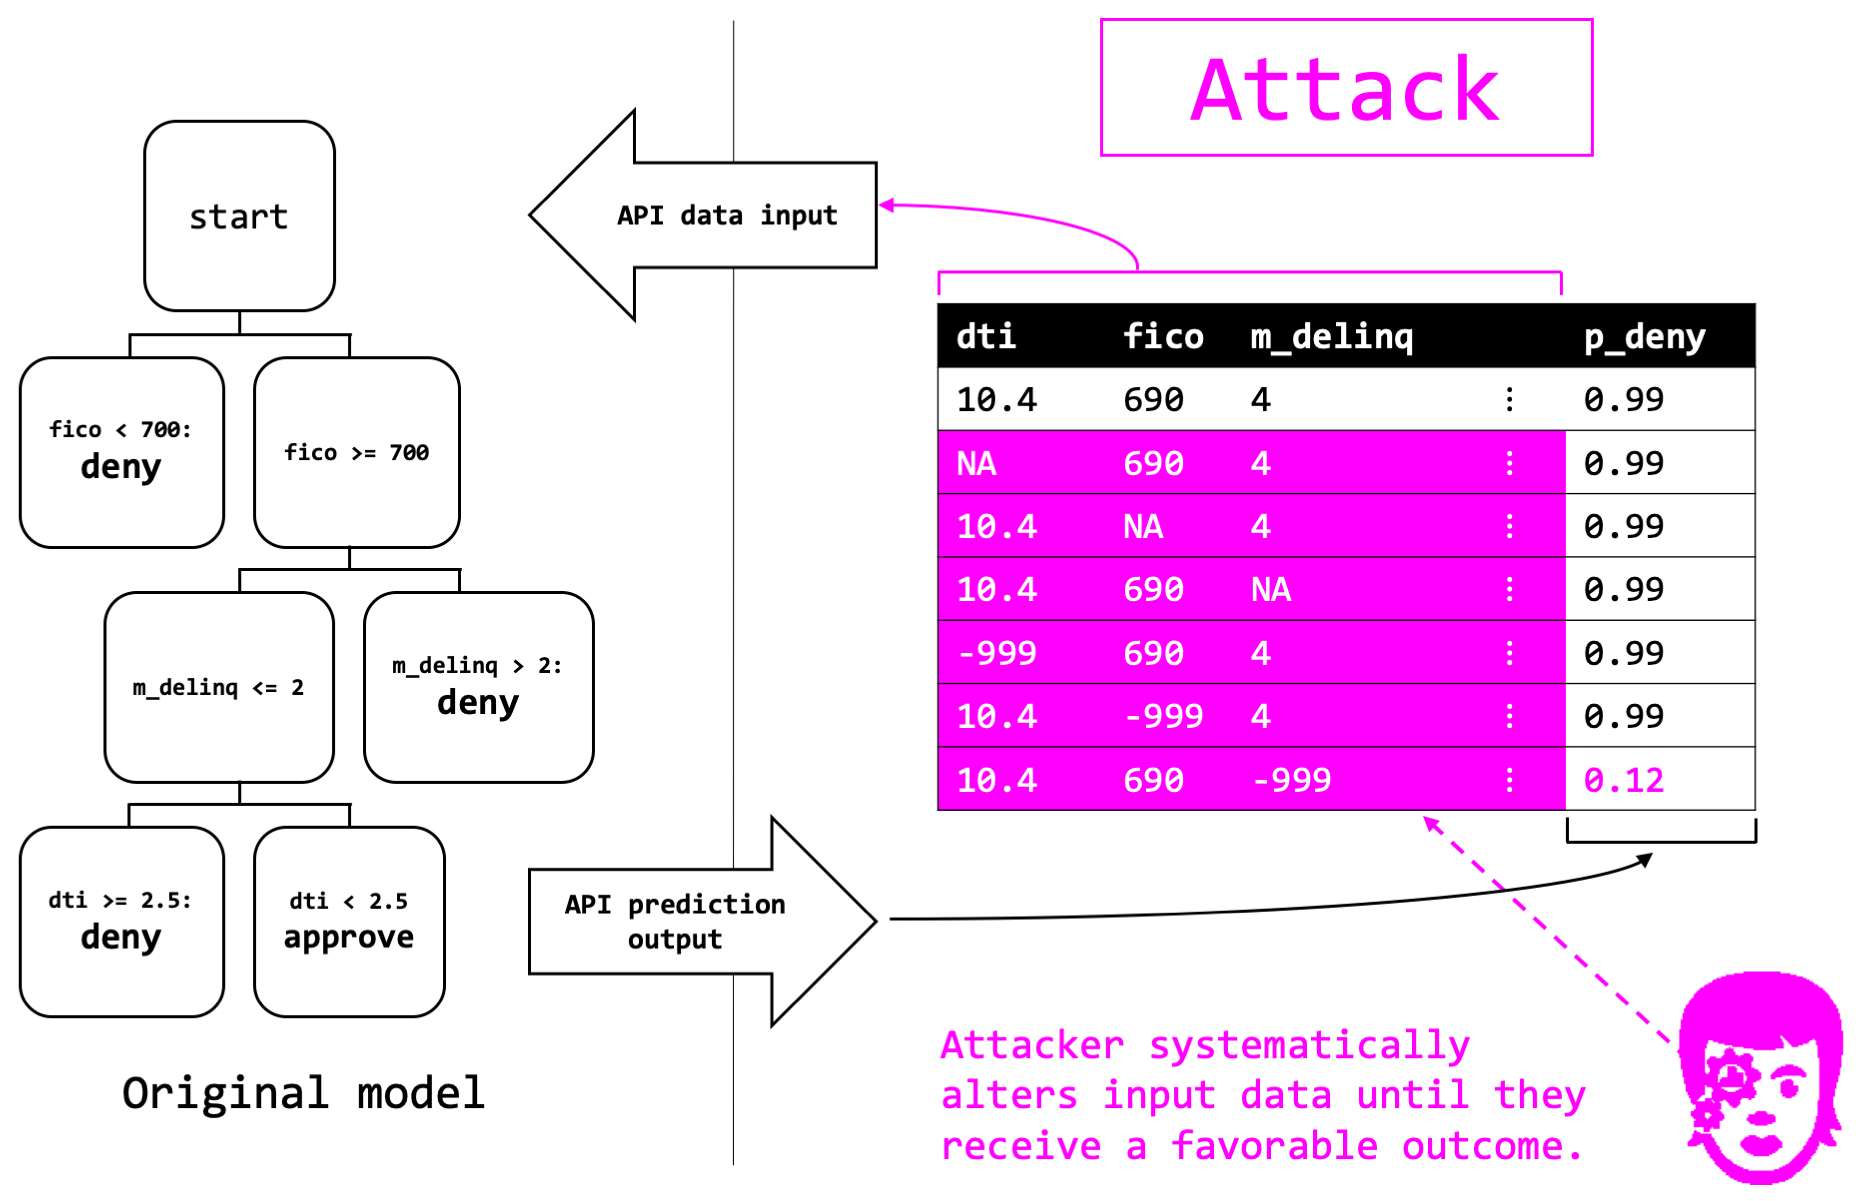
\includegraphics[height=135pt]{img/adversary.PNG}
				\end{center}
			\end{figure}	

		
		\end{frame}	

%-------------------------------------------------------------------------------
	\section{Impersonation}
%-------------------------------------------------------------------------------
	
		\begin{frame}
		
			\frametitle{Impersonation Attacks}		
			
			\begin{figure}[htb]
				\begin{center}
					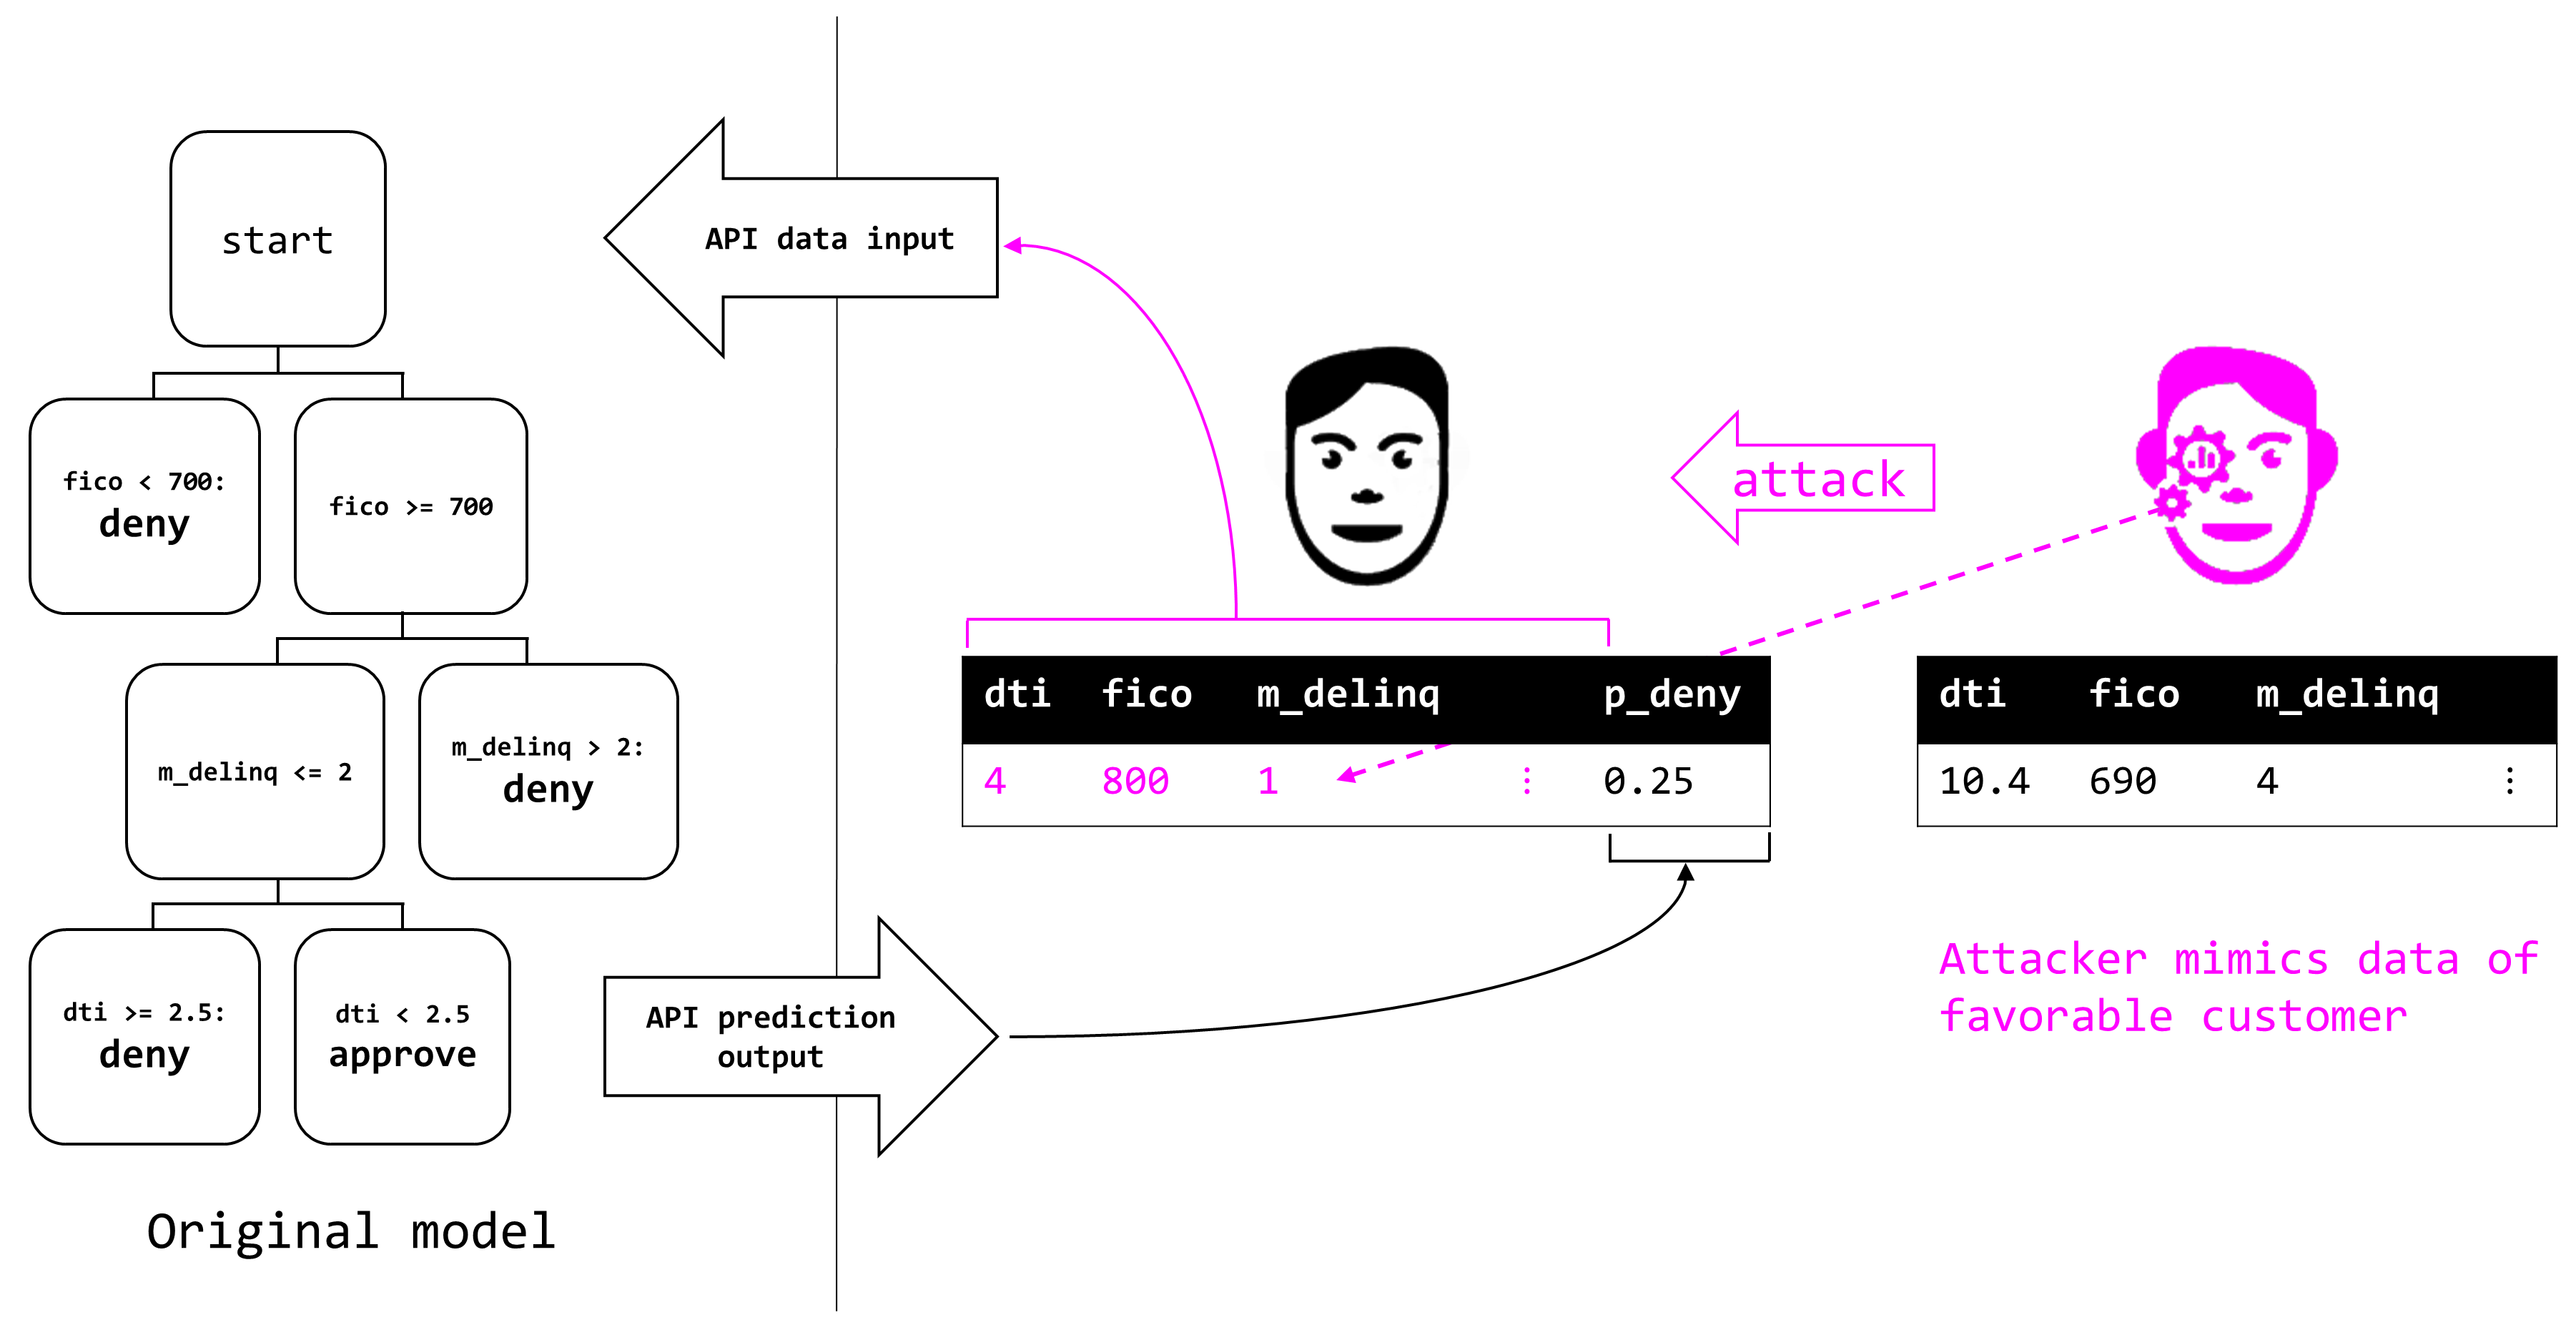
\includegraphics[height=135pt]{img/imperson.PNG}
				\end{center}
			\end{figure}	

		
		\end{frame}

%-------------------------------------------------------------------------------
	\section{Blueprint}
%-------------------------------------------------------------------------------
	
		\begin{frame}
		
			\frametitle{A Blueprint for Low-Risk Machine Learning}		
			
			\begin{figure}[htb]
				\begin{center}
					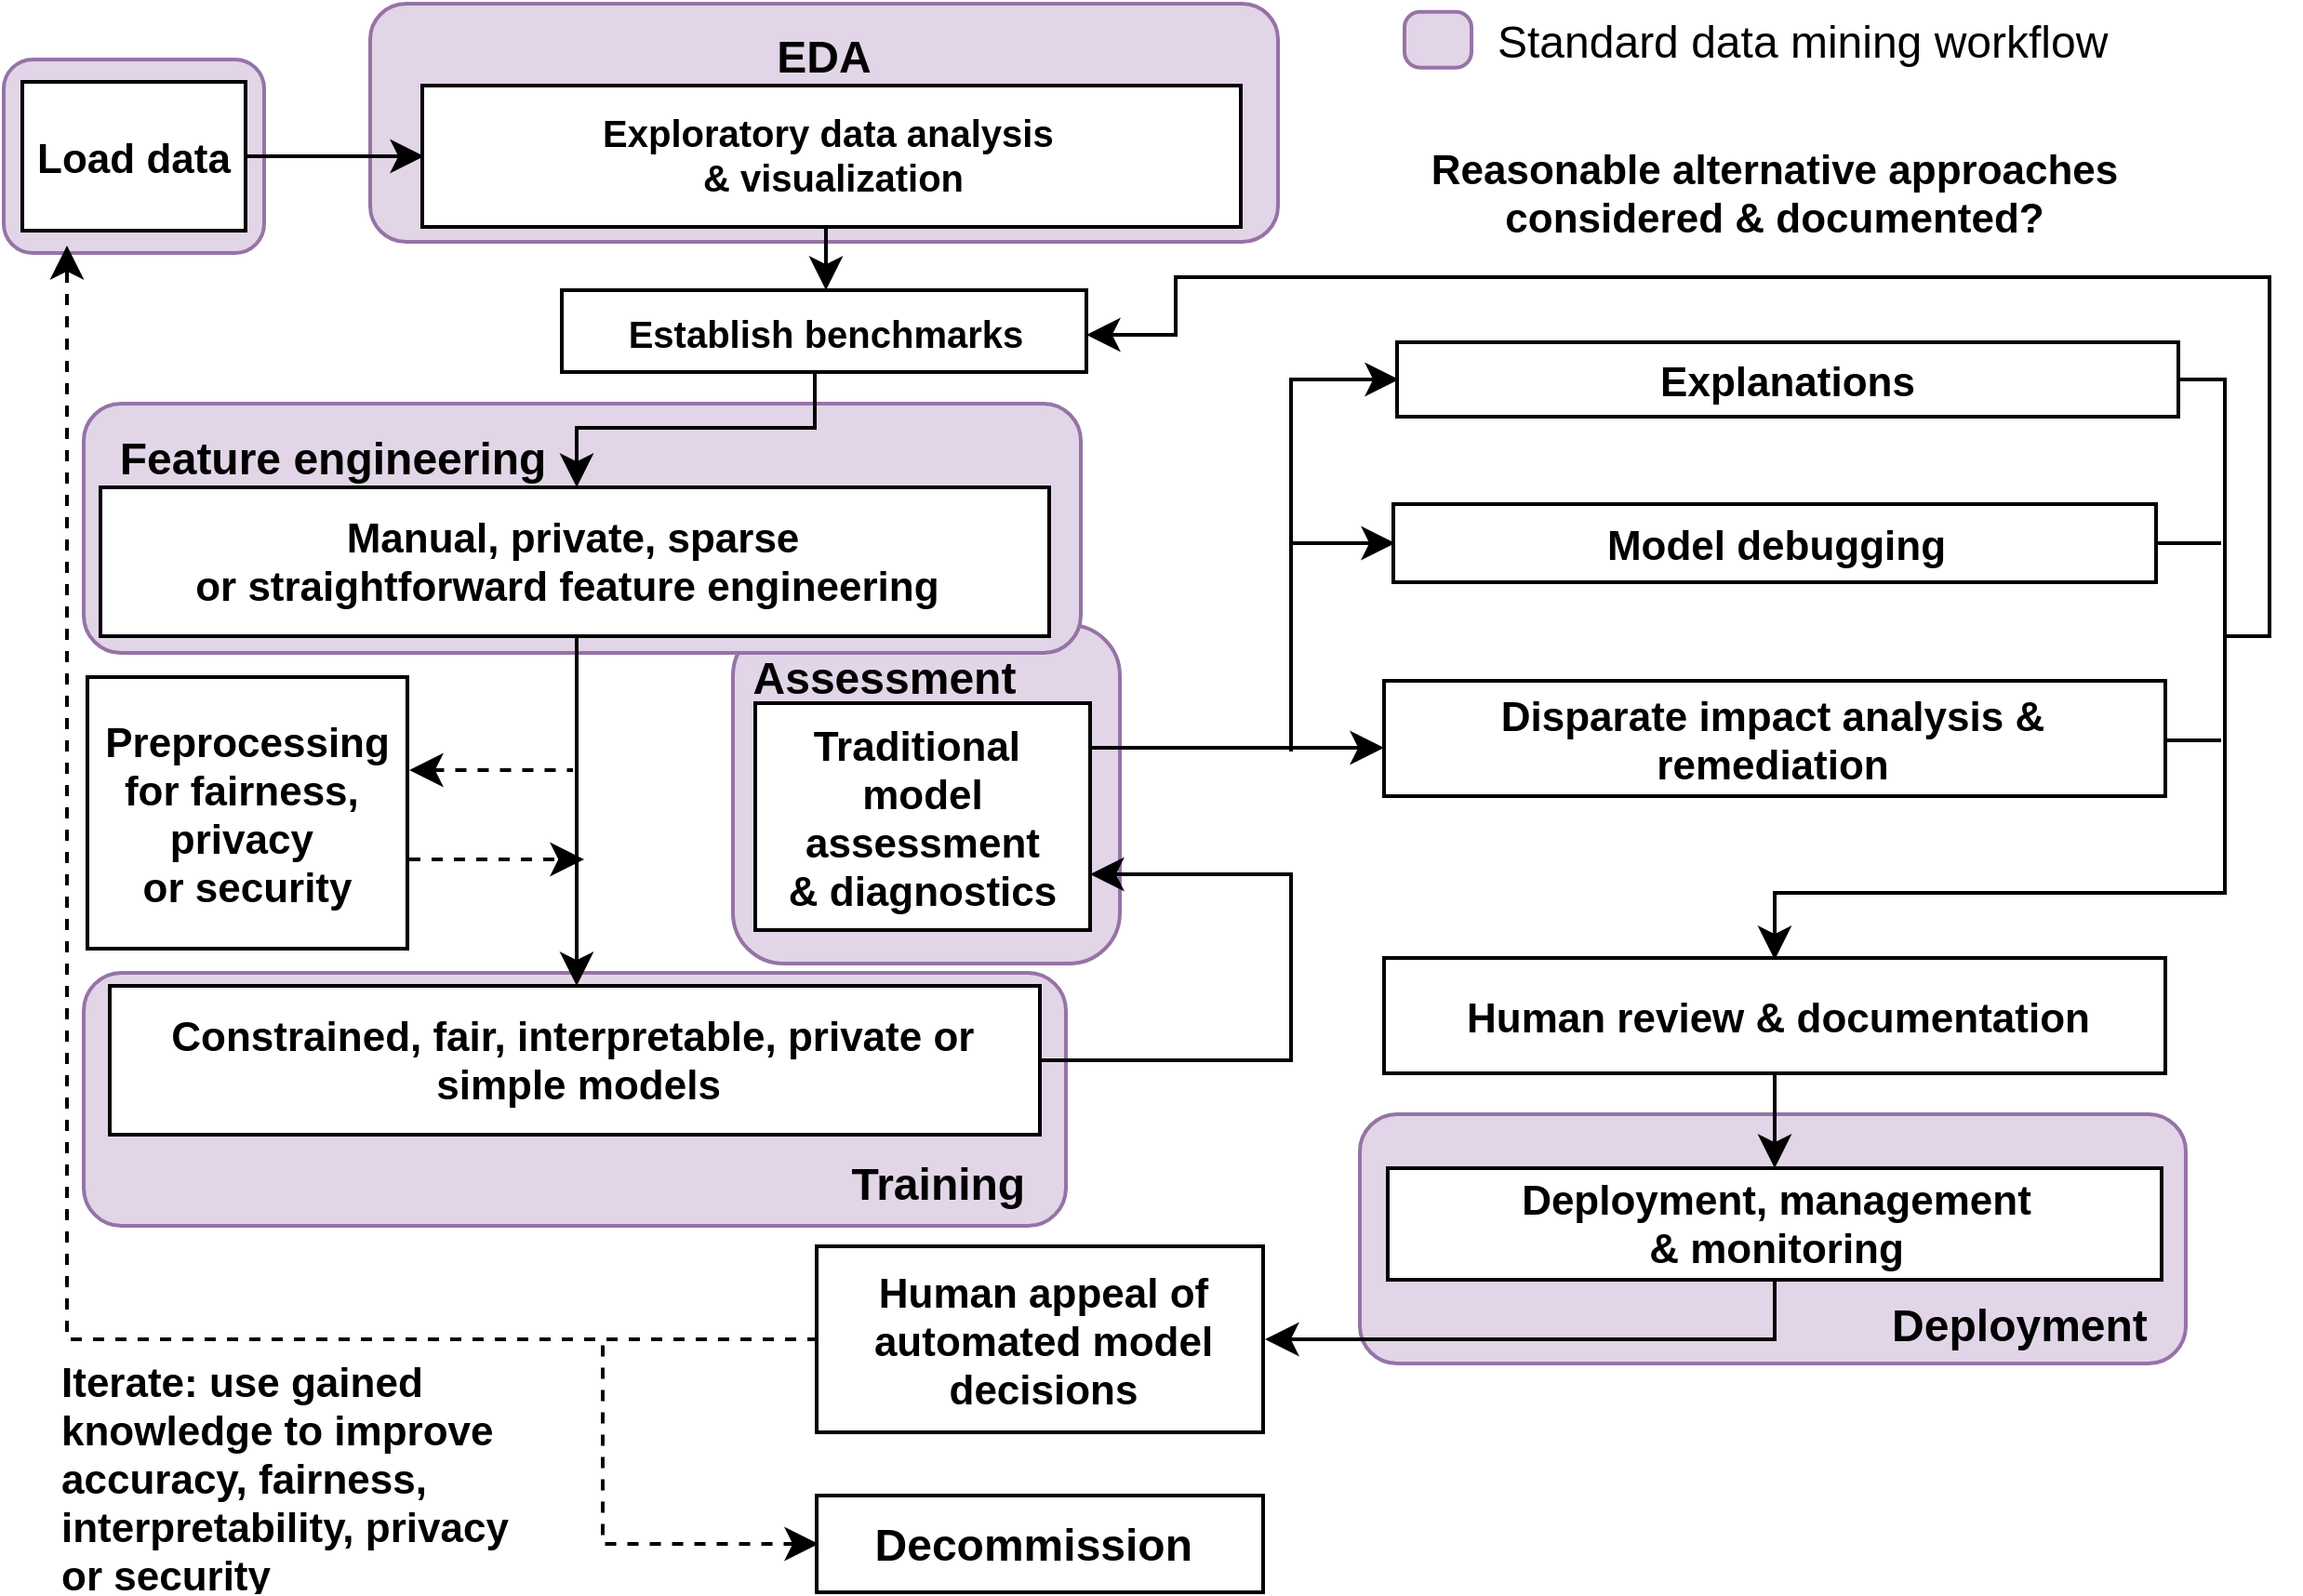
\includegraphics[height=135pt]{img/blueprint.png}
				\end{center}
			\end{figure}	

		
		\end{frame}

%-------------------------------------------------------------------------------
%	References
%-------------------------------------------------------------------------------

	\begin{frame}[t, allowframebreaks]
	
		\frametitle{References}	
		
			\textbf{Proposals for model vulnerability and security:}\\
			\small{\url{https://www.oreilly.com/ideas/proposals-for-model-vulnerability-and-security}}
			
			\vspace{10pt}
			
			\textbf{Can Your Machine Learning Model Be Hacked?!:}\\
			\small{\url{https://www.h2o.ai/blog/can-your-machine-learning-model-be-hacked/}}
			
		
		\framebreak		
		
		\printbibliography
		
	\end{frame}

\end{document}